%!TEX root = ../thesis.tex

\chapter[introduction]{Introduction}\label{chp:introduction}
%
% SIZE: ~9 pages
%
% OUTLINE: Broad introduction to the topic.
% - Motivate the reader.
% - Why should they care about this topic? 
% - What is the historical context of decision support, what are the practical implications of it, and what happens when it fails.

% \todo[inline]{Lead-in with conversations and the patient interview and how it affects the patient journey. How healthcare has seen rapid advances in medicine and medical devices for diagnostics and treatment but the patient interview and triaging has seen little development.}

In an era where technology increasingly intertwines with healthcare, artificial intelligence is on the verge of becoming part of standard medical practice. 
Growing administrative burdens, aging populations, and rapid scientific progress in medicine and medical devices have created a need to rethink how medical professionals are best enabled to successfully do their job. 
The application of artificial intelligence in medical decision-making is likely to hold significant potential to reduce the effect of these issues and improve patient outcomes \parencite{shailaja_machine_2018}. 
However, as such decisions impact critical aspects of human health and well-being, this prospect has also raised concerns relating to the reliability of systems that use artificial intelligence \parencite{chen_ethical_2021, ahmad_interpretable_2018}.

The use of technology to support decision-making can be traced back to very beginning of recorded history. After the agricultural revolution, several ancient civilizations developed mathematical techniques and algorithms to help them manage the newfound complexity of society. 
Fittingly, the first human name recorded in written history belonged to Kushim, a Sumerian accountant. Their signature has been identified on at least 18 clay tablets dated to 3400-3000 BCE, documenting transactions and inventory related to barley and other ingredients used in beer production \parencite{nissen_archaic_1993}. 
% A later example is the Egyptian Rhind Mathematical Papyrus dated to around 1550 BCE which describes various mathematical techniques for doing calculations involving multiplication, division, and fractions, and how to use them for practical purposes like measuring land, constructing buildings, and sharing resources \parencite{georges_universal_2001}. 
Later, the Babylonians developed a sophisticated system of mathematics that included algorithms for solving quadratic equations and calculating areas of shapes, and numerical methods for approximating square roots \parencite{fowler_square_1998}. 

Besides enabling the advancement of early society, these technologies also brought with them novel challenges. 
In a likely attempt to ease the strenuous work of doing Sumerian mathematics, Kushim produced a clay tablet with a multiplication table that included fractional representations of common numbers (\cref{fig:kushim_multiplication}). Assumedly unbeknownst to Kushim, this tablet would also come to contain one of the world's first recorded examples of a mathematical error; the statement: $5 \times \sfrac{1}{2} = 5$ \parencite{nissen_archaic_1993}. 
Later, the scribe of the Plimpton 322 clay tablet also made several errors when listing Pythagorean triplets, presumably struggling to grapple with Babylonian mathematics \parencite{neugebauer_mathematical_1945,britton_plimpton_2011,cuneiformdigitallibraryinitiativecdli_mct_2005}. 
% Later, in its list of Pythagorean triplets, the Plimpton 322 clay tablet (\cref{fig:plimpton_332}) also has several errors, presumably made by a novice in Babylonian mathematics \parencite{neugebauer_mathematical_1945,britton_plimpton_2011}. 
% Apart from such inherent limitations of the tools, inadequate human proficiency in their use was also a source of error. 
Besides these human errors, limitations inherent to the tools themselves also posed problems. 
The Babylonian number system, for instance, was well-equipped to represent rational numbers but inefficient at approximating irrational numbers. 
This forced significant approximation errors such as the common practice of approximating $\pi$ with 3 \parencite{georges_universal_2001}. 
% Easy to overlook, the challenges we face in adopting new technologies today are not new but have been faced by humans for thousands of years. Today, as in ancient times, it was important to understand the limitations of technology and the need for human expertise in its use.

% Yes, Babylonian mathematics, which developed in ancient Mesopotamia (modern-day Iraq) around 2000 BCE, had a numerical system that was capable of representing some irrational numbers, although they did so indirectly. The Babylonians primarily used a base-60 positional numeral system, which was well-suited for representing many rational numbers.

% Irrational numbers, such as the square root of 2 (√2) or π (pi), cannot be exactly represented in any finite numerical system, whether it's base-10 (our modern decimal system) or base-60 (used by the Babylonians). However, the Babylonians were able to approximate these irrational numbers to a certain degree using their sexagesimal system.

% For example, to approximate the square root of 2, the Babylonians might have used a fraction like 1;24,51,10 (where the semicolon represents the sexagesimal radix point). This would represent an approximation of √2, although not an exact representation. Similarly, they could approximate π using a sexagesimal fraction, but it would be an approximation rather than an exact value.

% The Babylonians were skilled mathematicians and astronomers, and they used their numerical system to perform a wide range of calculations, including those involving geometry and timekeeping. While they couldn't precisely represent irrational numbers, they could work with these numbers to a certain level of accuracy within the constraints of their base-60 system


% \begin{figure}[t]
%     \centering
%     % 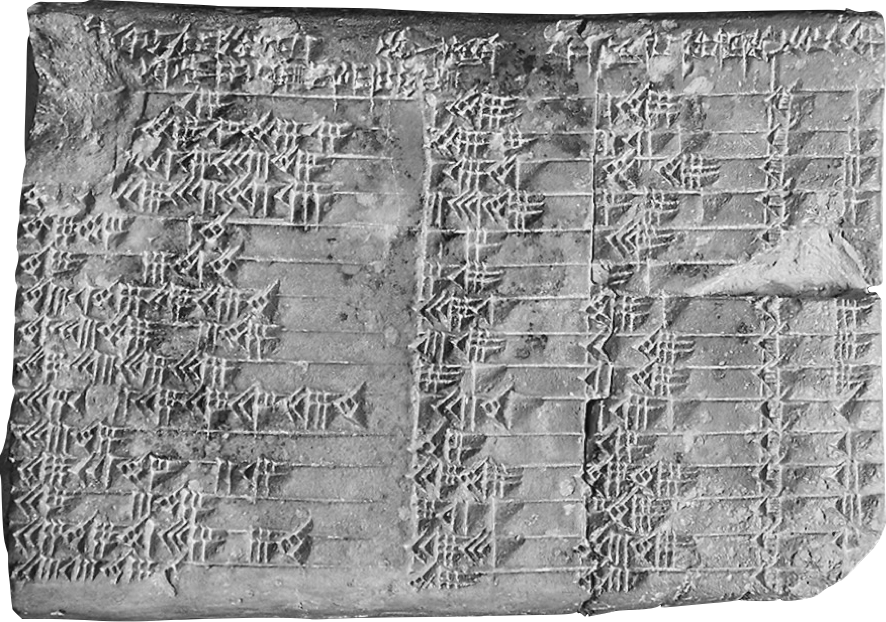
\includegraphics[width=0.90\textwidth]{plimpton_322.png}
%     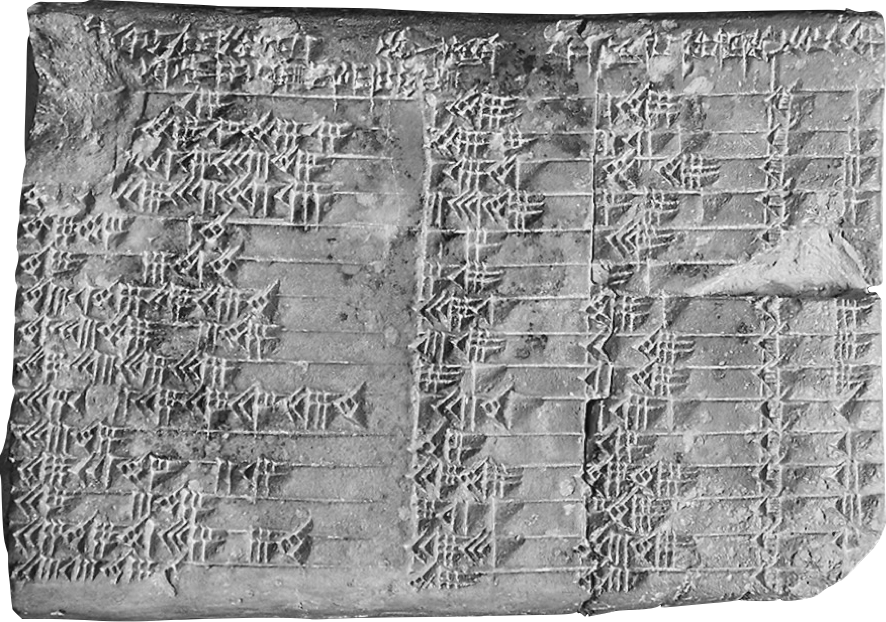
\includegraphics[height=0.4\textheight]{plimpton_322.png}
%     \caption[Technology is difficult. The scribe of the Plimpton 322 clay tablet ($\sim$1800 BCE) made several errors when listing Pythagorean triplets.]{ Technology is difficult. The scribe of the Plimpton 322 clay tablet ($\sim$1800 BCE) made several errors when listing Pythagorean triplets, presumably struggling to grapple with Babylonian mathematics. \parencite[photo credit][]{neugebauer_mathematical_1945, cuneiformdigitallibraryinitiativecdli_mct_2005}}
%     \label{fig:plimpton_332}
% \end{figure}

\begin{figure}[t]
    \centering
    % 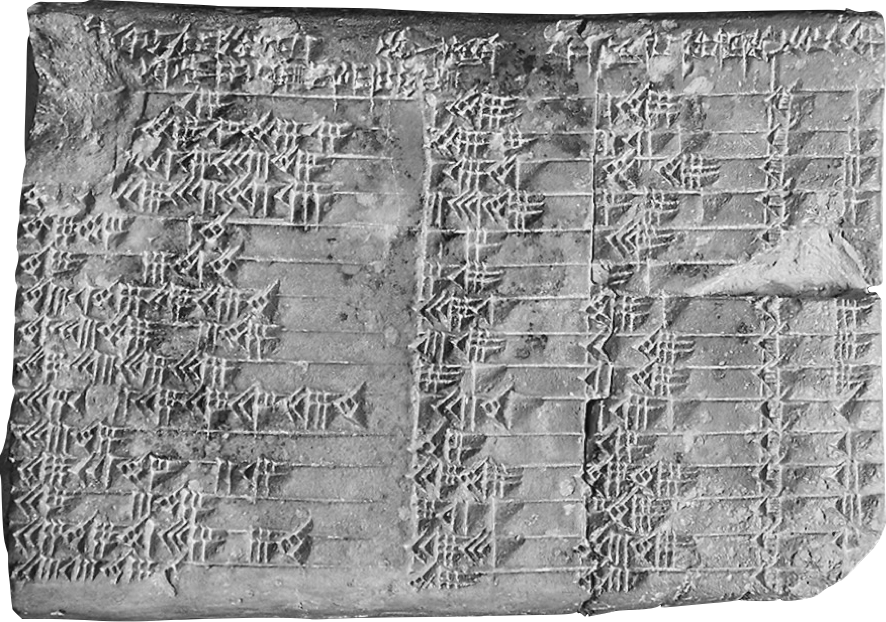
\includegraphics[width=0.90\textwidth]{plimpton_322.png}
    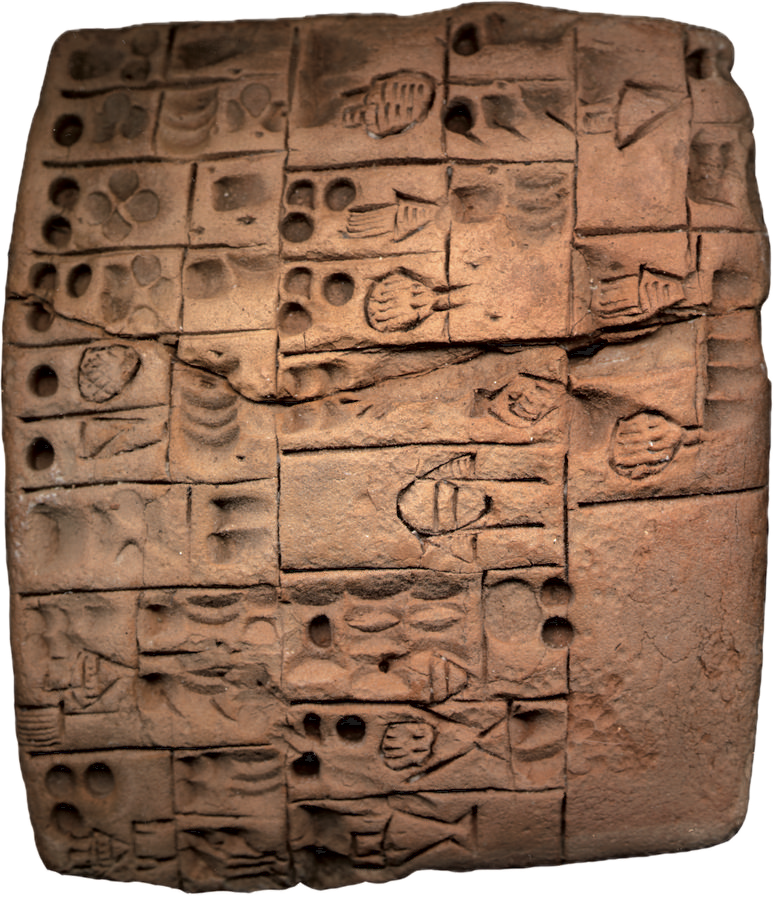
\includegraphics[height=0.55\textheight]{kushim_multiplication.png}
    \caption[Technology is difficult. The accountant Kushim made mistakenly claimed $5 \times \sfrac{1}{2} = 5$.]{ Technology is difficult. Between 3400 and 3000 BCE, the Sumerian accountant Kushim wrote this tablet. Besides calculations of basic ingredients required for the production of cereal products, in the top left $6 \times 2$ grid it contains a multiplication table. While presumably aimed to ease the strenuous work of doing Sumerian mathematics, unfortunately, the top row states: $5 \times \sfrac{1}{2} = 5$, an unforgiving imprint the worlds first recorded mathematical error \parencite{nissen_archaic_1993, renn_learning_2019}, \parencite[photo credit][]{cuneiformdigitallibraryinitiativecdli_msvo_2018}.}
    \label{fig:kushim_multiplication}
\end{figure}

While efforts to ease human decision-making have been ongoing for thousands of years, it was not until 1642 that the first mechanical calculator was successfully designed by Blaise Pascal. Refined by Gottfried Leibniz during the latter half of the 17th century, the mechanical calculator marked the beginning of a new era where rudimentary calculations could be automated and performed with greater speed and accuracy than by humans alone. 
In the 1820s, Charles Babbage proposed the first programmable mechanical computer, the Difference Engine. Although never completed, it laid the foundation for his later design of the Analytical Engine in 1837 which is considered to be the first general-purpose computer design. 
Working with Babbage, Ada Lovelace is widely regarded as the first to have recognized that programmable computers could have applications beyond pure arithmetic. However, only with the advent of electronics were the first successful general-purpose computers built, starting with the ENIAC in 1945 (\cref{fig:eniac_programmers}).
% While the potential of a general-purpose programmable computer with applications beyond pure arithmetic was recognized by Ada Lovelace,  
% it was not until the 1940s and 50s that % / 
% it took one-hundred years before / 
% the first programmable, electronic, general-purpose digital computers were developed, starting with the ENIAC in 1945 (\cref{fig:eniac_programmers}) \parencite{georges_universal_2001}. 
As the technology matured and manufacturing processes were refined and scaled, electronic computers were adopted widely across society for various applications in science and industry, including healthcare \parencite{georges_universal_2001, harari_sapiens_2011}.
% The societal changes brought about by the widespread adoption of computer technology through the latter half of the 20th century were so profound that some scholars refer to the era as the information age \parencite{georges_universal_2001, harari_sapiens_2011}.

\begin{figure}[t]
    \centering
    % 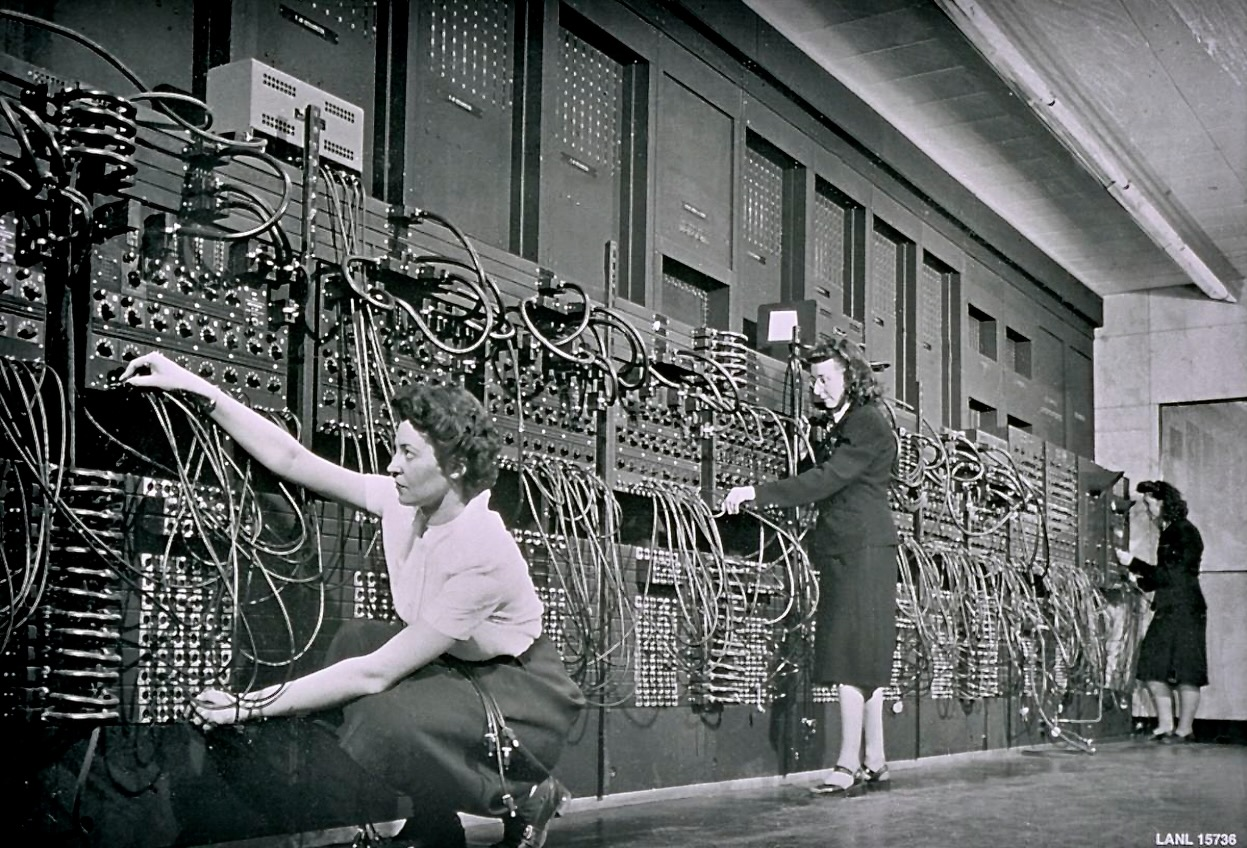
\includegraphics[width=0.95\textwidth]{eniac_programmers.jpeg}
    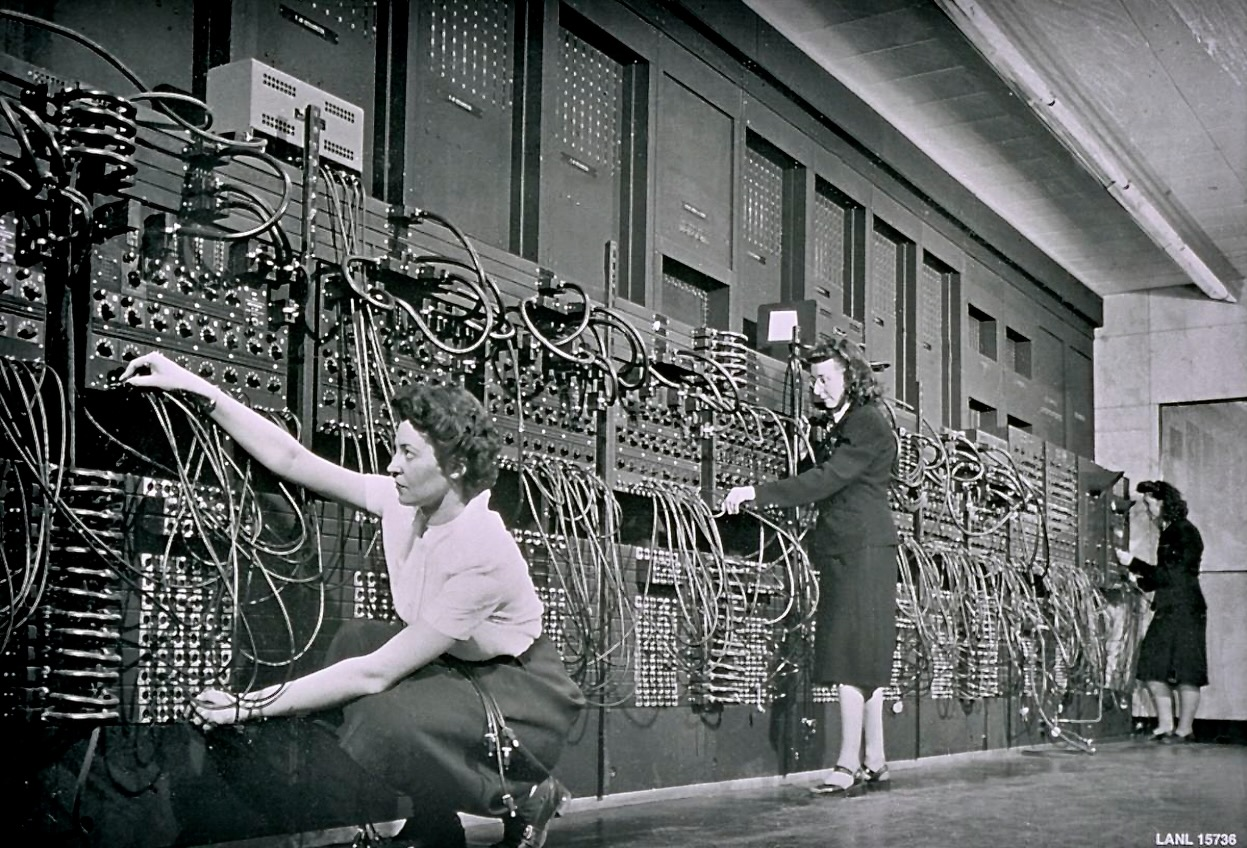
\includegraphics[height=0.42\textheight]{eniac_programmers.jpeg}
    \caption[Ruth Lichterman (left) and Marlyn Wescoff (middle) were two of the several female programmers of the ENIAC, the world's first general-purpose electronic computer.]{ Ruth Lichterman (left) and Marlyn Wescoff (middle) were two of the several female programmers of the ENIAC. \parencite[photo credit][]{usarmyresearchlaboratoryarltechnicallibrary_female_1940}}
    \label{fig:eniac_programmers}
\end{figure}

With the digital revolution continuing into the 21st century and the worldwide spread of the internet, the amount of data and its availability have grown exponentially. 
This has led to a surge of interest in the scientific field of machine learning, a subfield of artificial intelligence, that studies how computer algorithms can learn functions from data and make predictions to guide decision-making. 
Enabled by a massive increase in the performance and availability of parallel computing resources, such methods have set new standards for the abilities of computer systems at various tasks usually reserved for humans, such as vision, speech recognition, and natural language understanding \parencite{lecun_deep_2015}. 
In recent years, machine learning has also made its way into healthcare systems, where it has shown promising results on difficult tasks such as medical imaging \parencite{lundervold_overview_2019}, drug discovery \parencite{chen_rise_2018}, and clinical decision support \parencite{cite15, cite14}. 

\begin{figure}[t]
    \centering
    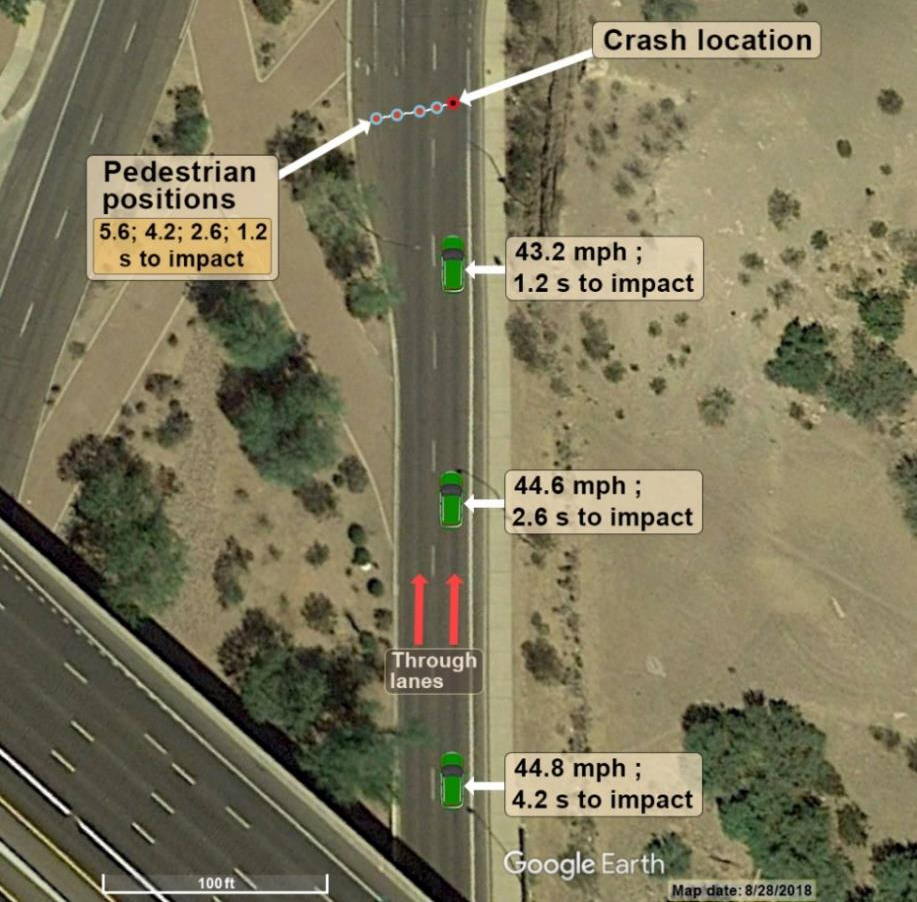
\includegraphics[width=0.85\textwidth]{uber_nhsa_accident_cropped.png}
    \caption[A pedestrian was killed by an Uber self-driving car in Tempe, Arizona in 2018.]{ A pedestrian was killed by an Uber self-driving car in Tempe, Arizona in 2018. The car's sensors detected the pedestrian $5.6$ seconds before the crash, but the self-driving system failed to recognize its own uncertainty in multiple object misclassifications and so did not correctly predict her path or reduce the SUV's speed \parencite[photo credit]{nationaltransportationsafetyboardnhsa_collision_2019}.}
    % \caption{Aerial view of crash location showing path of pedestrian as she attempted to cross N. Mill Avenue and movement and speed of SUV at three points before impact. Pedestrian's path shows her position from initial detection ($5.6$ seconds before impact) until impact; SUV's position is shown at corresponding times beginning $4.2$ seconds before impact \parencite{nationaltransportationsafetyboardnhsa_collision_2019}.}
    \label{fig:uber_nhsa_accident}
\end{figure}

% While machine learning has immense potential for positive impact, as any of it also comes with risks of error, much the same as its predecessors. 

% While applications in healthcare are `nascent' and generally move forward slowly, machine learning has been fast adopted for self-driving vehicles. 

% As with other technologies that came before it, limitations of the machine learning itself, human error, and the complexity of the real world are all factors that can lead to failures. 
% However, compared to earlier, the sheer number of potential applications of machine learning, and the weight of some of them, serve to amplify both potential benefits and risks.

% As for all technologies that came before it, limitations of machine learning algorithms, the complexity of the real world, and human error can all lead to failures. 
% As for all technologies that came before it, machine learning systems can result in error, whether due to the complexity of the real world, human error, or limitations inherent itself.

% However, the vast array of applications and their large potential impact amplifies these effects, compared to earlier technologies. 

% Similar to technologies that came before it, machine learning brings risks alongside its benefits. 
% % The complexity of the real world, limitations inherent to machine learning itself, and human mistakes can all lead to errors, while the nature of some applications serves to amplify their consequences, compared to some earlier technologies. 
% % Real-world complexity, limitations of machine learning itself, and human error can all lead to system errors whose consequences might be amplified compared to earlier technologies due to the nature of some applications, such as in healthcare or autonomous driving.
% % Real-world complexity, machine learning limitations, and human errors can magnify risks in fields like healthcare and autonomous driving
% Risks, as well as benefits, might be amplified in machine learning compared to earlier technologies due to the nature of some of the tasks that machine learning enables augmenting.
% While applications in healthcare are nascent and generally move forward in small steps, autonomous driving has fast adopted machine learning and presents a pertinent example: 

Machine learning, like previous technologies, carries both benefits and risks. 
However, machine learning might exacerbate some of these risks due to the unique tasks it enables in domains such as healthcare and autonomous driving. 
While applications in healthcare are nascent and generally move forward in small steps, autonomous driving has fast adopted machine learning and presents a pertinent example: 
% A pertinent example is autonomous driving systems which were fast equipped with machine learning technology: 
In 2018, the first incident of a self-driving car killing a pedestrian took place in Tempe, Arizona. 
The car, an SUV operated by Uber, was driving in autonomous mode when it struck a pedestrian crossing the street with her bicycle. 
According to the investigation by the National Transportation Safety Board, the car's sensors detected the pedestrian more than five seconds before the crash, but the system did not manage to correctly predict her path or reduce the SUV's speed. 
Specifically, during those seconds, the system incorrectly classified the pedestrian more than ten times, first as a vehicle, then as an unknown object and ultimately as a bicyclist, each time changing, or resetting, the pedestrian's predicted path. 
About one second before the crash, the system determined that a collision was imminent, but the situation exceeded the constraints within which the autonomous driving system was allowed to operate, and the car's safety driver failed to intervene (\cref{fig:uber_nhsa_accident}) \parencite{nationaltransportationsafetyboardnhsa_collision_2019}. 
%
And Uber is not the only actor facing the challenges of applying machine learning in real-world scenarios. A recent report by the Washington Post found that Tesla's Autopilot system has been activated during at least 736 crashes in the last four years with 16 fatalities \parencite{siddiqui_17_2023}. 
% And though recent statistics published by Waymo, 
% %the self-driving car company owned by Google's parent company Alphabet, 
% revealed far fewer crashes, with only 2 of 20 incidents over 1 million miles meeting reporting criteria, it is interesting to note that the cars are all operated in the sunny states of California and Arizona, where driving conditions vary relatively little \parencite{hawkins_waymo_2023}. 
While driver-assistance systems undoubtedly help reduce accidents in many cases, and humans have been argued to be worse drivers still, the issues of current systems highlight the need for machine learning systems that are robust in rare, adverse, and difficult situations \parencite{metz_how_2022}. 
% While driver-assistance systems undoubtedly help reduce accidents in many cases, and has great future potential, the issues of current systems highlight the need for machine learning systems that are robust in rare, adverse, and difficult situations. 

Recently, European policymakers proposed legislation to enforce that applied machine learning meets certain standards \parencite{europeancommission_briefing_2021}. 
This so-called AI Act considers three categories of applications based on the potential risk they pose to society: limited, high, and unacceptable. 
Autonomous vehicles and systems within healthcare fall in the category of high risk applications. To avoid critical errors, these must meet a set of strict requirements focusing on anti"-discrimination and robustness.
% Limited risk applications such as in computer games must meet transparency criteria, while
% Facial recognition is an example of an application deemed to pose unacceptable risk to society.
% Limited risk applications, such as in computer games, must meet transparency requirements, and technologies such as public facial recognition are banned due to unacceptable risk. 

% Miscalibrated models are unreliable, especially in high risk applications, and although no model is perfect, the inability of a human, or a model, to assess the certainty with which a prediction was made, makes it impossible to know how to weigh it in a decision-making process. 
% A connection can be made back to the incident with the Uber self-driving car. 

One of the key advances needed to ensure that high-risk applications of machine learning comply with such requirements is accurate uncertainty estimation of machine predictions. 
The multitude of rapid misclassifications made by the Uber self-driving car in Tempe is a likely indication that the model responsible for object-classification was overconfident in its predictions and unable to represent or communicate this uncertainty to other subsystems in the car, or the safety driver. 
As a consequence, the model's many incoherent predictions were taken at face value and other subsystems acted on them without appropriate consideration to their reliability.
While any model will inevitably make wrong predictions, accurately estimating the associated uncertainty and communicating it to reliant systems or humans is necessary to reduce the risk that wrong predictions lead to catastrophic failures. 
Fittingly, a recent study by the European Parliamentary Research Services \parencite{europeanparliament_artificial_2022} concluded: 
%
\begin{quote}
    \centering\itshape
    Future AI solutions for healthcare should be implemented by integrating uncertainty estimation, a relatively new field of research that aims to provide clinicians with clinically useful indications on the degree of confidence in AI predictions.
\end{quote}
% \vspace{0.5em}
\begin{center}
\noindent\rule{0.2\textwidth}{0.5pt}
\end{center}
\vspace{1em}
%
%
% OUTLINE: Primer overview of the thesis. What are the topics and what is the context of the research.
% \noindent The research presented in this thesis will focus on the use of machine learning in relation to uncertainty estimation, speech processing, and medical conversations. 
\noindent The research presented in this thesis deals with the use of machine learning for medical interviews with a focus on uncertainty estimation and representation learning. 
The research project was partially funded by a grant from the national Danish Innovation Fund (grant no.\@ 0153-00167B) and defined and carried out in collaboration with the Danish health tech company Corti, which develops computer software for medical decision support. 
In the rest of this chapter, we will provide a high-level introduction to these topics, and to Corti, and discuss the motivation behind the research project.


\section{Uncertainty by example: Corti use-cases}
%
% OUTLINE: Motivate the research project. 
% - What is the context of the research and why is it important? 
% - What are the current applications of machine learning in the domain (decision support in healthcare)?
% - What are the practical implications of the research? 
% - What are the challenges and limitations of the current state-of-the-art?
%
Corti develops decision support software for healthcare professionals such as general practitioners, medical coders, and call-takers at emergency medical services. The system supports the professional similar to a copilot for medical interviews, for instance providing a graph-based protocol for triaging and helping to keep track of key information shared in the conversation. 

When used by emergency services for example, calls are transcribed in real-time using automatic speech recognition built for the customer-domain and the system makes suggestions for the call-taker to use in the conversation with the caller, including notifications about forgotten protocol questions \parencite{havtorn_multiqt_2020} and potential cases of cardiac arrests \parencite{cite15, cite14}. The system logs the details about the call and the actions taken by the call-taker for later use in review, training and quality assurance. 

% - a copilot for medical interviews
% - decision support
% - quality assurance
% - documentation
% -> many applications


\subsection{Stroke recognition in emergency calls} \label{subsec:motivation-stroke-recognition}
%
\paragraph{Case background} In 2021, Corti entered a research collaboration with the Capital Region of Denmark and the Copenhagen Emergency Services to develop a system for recognizing stroke cases in calls to the 1-1-2 emergency line and the 1813 medical helpline. 
Stroke is one of the biggest causes of disability and death worldwide \parencite{cite1,cite2,cite3} and effective treatment is highly time-sensitive \parencite{cite4,cite5}. The most common gateway to specialized treatment and hospital admittance is through prehospital telehealth services like emergency medical call centers, nurse advice call lines, and out-of-hours health services \parencite{cite6,cite7}, however, studies have found that approximately half of all patients with stroke do not receive the correct triage for their condition from call-takers \parencite{cite10,cite11,cite12}. 
This is likely due to the complexity of stroke cases which exhibit a wide range of symptoms that can be difficult to recognize over the phone. Additionally, stroke cases are relatively rare, occurring in only $0.25\%$ of all calls made to the Copenhagen 1813 medical helpline in 2021. This makes it difficult for call-takers to gain practical experience with stroke cases which compounds to the fundamental difficulty of recognizing them. Although several efforts have been made to improve recognition rates, there is still a need for better tools to support call-takers in recognizing stroke cases \parencite{cite13,cite14,cite15}.

\paragraph{Uncertainty in stroke recognition} A reasonable machine learning pipeline to assist in recognizing stroke cases on calls to emergency services could consist of an automatic speech recognition model that transcribes the conversation and a binary classifier that estimates the probability that the transcript describes a case of stroke. 
Such a system might be trained on a dataset calls with verified stroke and non-stroke cases and evaluated against a held-out test set of calls where the call-taker has indicated whether they suspect a stroke. Due to the low prevalence of stroke cases, the dataset would be highly unbalanced, and the number of stroke cases limited. 
% The performance of such a system would depend on the quality of the automatic speech recognition model, the quality of the classifier, and the quality of the data used to train them. 
In such a system, many factors can lead to classification errors, and when that happens, we would like the model to express high degree of uncertainty. 
For instance, the automatic speech recognition model might make an error in the transcription of particular word or phrase due to a noisy environment, overlapping, slurred or mumbling speech, or words not in the model's training data. 
The classifier might misclassify a conversation due to medically ambiguous symptoms, a general lack of information given in the conversation, or transcription errors made by the speech recognizer. 
How to best make such models accurately represent and estimate the uncertainty of given predictions, and how to use it to improve the value of such a system, especially in cooperation with the call-taker, is an open question.
What is clear, however, is that the ability of such a system to accurately estimate the uncertainty of given predictions is crucial for its safe and reliable deployment in the real world. Overconfident predictions could lead to unnecessary delays in treatment, misdiagnoses, increased costs for the healthcare system, and potentially fatal consequences for patients.


\subsection{Medical coding of clinical notes} \label{subsec:motivation-medical-coding}
%
\paragraph{Case background} During the course of this project, Corti's portfolio has expanded to include a software system for medical coding of clinical notes. 
When a patient is admitted to a hospital, the medical staff will write a clinical note describing the patient's diagnosis and the procedures they underwent, including drug prescriptions. 
These notes are then used for billing and reimbursement purposes, as well as for research and quality assurance. 
The clinical notes are written, usually by a doctor, in natural language adhering to a certain structure. Later, a medical coder will assign a set of codes to the note based on its content. 
The process of medical coding is time-consuming and error-prone due to the vast number and high complexity of medical diagnoses and procedures. For instance, the widely used International Classification of Diseases (ICD) standard consists of 55,000 medical codes in version 10 and 85,000 in version 11 \parencite{worldhealthorganisationwho_international_2023}. Additionally, a single clinical note will usually contain several diagnoses and procedures which must all be inferred from the natural language text \parencite{johnsonMIMICIIIFreelyAccessible2016,johnsonMIMICIVFreelyAccessible2023}. 
Furthermore, any single code can have several criteria defined by official guidelines that determine under which conditions it is mutually exclusive with other codes, and when other codes must be coded along with it \parencite{centersformedicaremedicaidservicesus_icd10cm_2023}. These properties make medical coding a very complex, multi-label classification problem. 
% Official guidelines describe how to code specific diagnoses and procedures and combinations thereof . 
% For instance, a code may have several exclusion or inclusion criteria which define which other codes must be coded along with it, or when they must not. 

\paragraph{Uncertainty in automated medical coding} A reasonable machine learning pipeline to assist in medical coding could consist of a natural language processing model that extracts relevant information from the clinical note and outputs a probability distribution for each of the potential medical codes. 
However, training and using such as system comes with several challenges. 
For instance, the prevalence of different medical codes in the training data is highly unbalanced; it is common to have several orders of magnitude difference between the frequency of the most frequent code and the least frequent code. Since each clinical note is associated with multiple codes that have complex co-occurrence patterns, it is often impossible to exactly correct for this class imbalance by stratified sampling, which is the usual go-to approach to deal with class imbalance in machine learning. 
% This also gives rise to 
Furthermore, some codes are highly similar, for instance the ICD-10 codes Z87.891 ``Personal history of nicotine dependence'' and F17.210 ``Nicotine dependence, cigarettes, uncomplicated''. In practice, however, only one of them should be assigned to a given note. 
As with the stroke recognition system, we would like the model to express high degree of uncertainty when it makes a mistake. For example, if the model is uncertain about two similar codes, it might be appropriate to ask a human expert to review the note and make the final decision. Additionally, the lack of training data for the rarest codes makes them difficult to learn to robustly predict, and so, we might reasonably expect the model to often be uncertain for rare codes. 


\section{Machine learning reliability} \label{sec:machine-learning-reliability}
%
Several factors define the reliability of a machine learning model. 
Besides model performance and accuracy, important factors include the \emph{interpretability} of how the model functions, the \emph{explainability} of its predictions, \emph{fairness} in its treatment of different groups, and \emph{robustness} to noise, outliers, and adversarial attacks. 
Since many modern machine learning models are deep neural networks with millions or billions of parameters, their size and complexity make them inherently difficult to interpret, and their predictions hard to explain. 
Due to high cost and practical infeasibility, the vast amounts of data needed to train such models are often not manually curated for quality, and so, may contain biases and errors which models are well-equipped to learn to mirror, risking fairness \parencite{burkart_survey_2021}. 
Finally, a number of factors, including the ability of deep neural networks to overfit, or even memorize, their training data \parencite{arpit_closer_2017, burg_memorization_2021}, can lead to models that are sensitive to adverse noise conditions and outliers. 

The ability of a model to accurately estimate the uncertainty of its predictions plays an important role in its reliability. While associating any prediction with an accurate uncertainty estimate can be argued to improve both interpretability, explainability, and fairness, the main goal is to improve the model's robustness to noise, outliers, and adversarial attacks. 
Given an input which cannot be mapped to a single output with certainty, the model can then indicate that its prediction should not to be trusted. 
However, overfitting, memorization, and the use of training objectives that are proxies for the evaluation metrics of interest often lead to models that are miscalibrated; that is, the predicted probability of a class does not reflect the true probability of the model being correct \parencite{guo_calibration_2017, kull_temperature_2019}. 
% This means, for instance, that if for a certain input the model assigns 70\% probability to a class, it would not generally be right 70\% of the time - if we could repeat the prediction multiple times under similar circumstances \parencite{guo_calibration_2017, kull_temperature_2019}.
Usually, the predicted probabilities are too extreme which leads to overconfident predictions. This means a model will often assign a high probability to the predicted class, even when it is wrong. 

% Miscalibrated models are unreliable, especially in high risk applications, and although no model is perfect, the inability of a human, or a model, to assess the certainty with which a prediction was made, makes it impossible to know how to weigh it in a decision-making process. 
% % A connection can be made back to the incident with the Uber self-driving car. 
% The multitude of rapid misclassifications made by the Uber self-driving car in Tempe is likely an indication that the model responsible for object-classification was overconfident in its predictions and unable to represent or communicate uncertainty to other systems in the car, or the safety driver. Instead, the model's predictions were taken at face value and subsystems in the car acted on them without appropriate consideration to their reliability.


\subsection{Model calibration} \label{subsec:model-calibration}
% 
The problem of miscalibration in machine learning models is well-known and has been studied for decades \parencite{lewis_sequential_1995, platt_probabilistic_1999, garczarek_classification_2002, zadrozny_transforming_2002, bennett_using_2003, niculescu-mizil_predicting_2005}. One of the best known methods for calibrating a binary classifier is Platt scaling which fits a logistic regression model to the model outputs, assuming that the miscalibration can be corrected by a logarithmic function \parencite{platt_probabilistic_1999}. Another method is isotonic regression which instead fits a nonparametric, monotonic function \parencite{zadrozny_transforming_2002}. 
More recently, \textcite{guo_calibration_2017} proposed a single-parameter variant of Platt-scaling that fits only a temperature parameter on the logits of a neural network classifier. 
These methods are generally simple and effective, but not without limitations. 
To perform the calibration, most of the methods require a held-out validation set on which the model was not trained, Platt scaling and isotonic regression are not directly applicable to multi-class classification problems, and how to calibrate models for structured prediction tasks, such as speech recognition and machine translation, remains an open problem \parencite{astudillo_uncertainty_2010, astudillo_integration_2013, jayashankar_detecting_2020}.

More importantly, correct calibration of a machine learning model does not guarantee that the predicted probability is accurate. 
Specifically, even a well-calibrated model can be overconfident for data that were not presented to it during training such as rare events, outliers, and adverse examples, sometimes collectively referred to as out-of-distribution examples. 
For instance, take a perfectly calibrated model trained to classify images of cats and dogs. If presented with an image of a horse, the model has no option but to distribute 100\% total probability across the cat and dog categories, even though that is clearly wrong. 
Worse yet, to indicate maximal uncertainty, we might expect the model to assign 50\% probability to each of the cat and dog categories, but sadly that behavior is not guaranteed. 
On the contrary, since no horses were in the training data, the model will not have learned specialized features for horses, nor learned to associate any relevant known features with horses. So, if a particular horse has features that resemble those learned for a dog more than for a cat, the model might assign arbitrarily high probability to the dog class; and vice versa. Therefore, even perfectly calibrated models risk being confidently wrong \parencite{zhou_survey_2022}. 


\subsection{Understanding uncertainty} \label{subsec:understanding-uncertainty}
% 
% OUTLINE: Introduce aleatoric and epistemic uncertainty. 
% - Discuss the distinction between them and how they relate to the problem of uncertainty estimation in machine learning.
% - 
% 
As hinted at in the previous section, there are different sources of uncertainty in machine learning models. 
At a fundamental level, we can decompose the \textit{predictive uncertainty} into uncertainty that is present in the knowledge we have, and uncertainty that originates from the knowledge that we do not have.
These sources are sometimes called \emph{known unknowns} and \emph{unknown unknowns}, or referred to in terms of \textit{aleatoric uncertainty} and \textit{epistemic uncertainty} \parencite{kendall_what_2017}. 
Aleatoric comes from the Latin word 'aleatorius' for 'dice player' or 'gambler' and refers to uncertainty present in the data itself due to randomness in the process that generated it. This kind of uncertainty is commonly seen as irreducible but, since it is represented in the collected data, it can usually be modelled directly. 
Epistemic comes from the Greek word 'epistḗmē' which means 'knowledge' and refers to uncertainty due to things one could in principle know, but does not in practice. Such lack of knowledge could for instance be due to a lack of data, or an improper model specification. 
Aleatoric uncertainty is sometimes referred to as \textit{stochastic uncertainty} and epistemic uncertainty as \textit{systematic uncertainty} \parencite{kendall_what_2017}. 
% Although the distinction between aleatoric and epistemic uncertainty is important, it is not always useful. For instance, a model may be uncertain about a particular prediction due to any of these two kinds of uncertainty. For that reason, the quantity of interest is usually the combined aleatoric and epistemic uncertainties, often referred to as \textit{predictive uncertainty}. 

An example of aleatoric uncertainty is the uncertainty in the transcription of a word due to a noisy environment or overlapping, slurred or mumbling speech. 
Unknown words are arguably sources of epistemic uncertainty although a good speech recognition model might generalize well if the word's spelling and pronunciation follow the same patterns as in the training data. Another example of epistemic uncertainty is the occurrence of truly out-of-distribution examples such as the horse in the image classifier example from earlier: inputs unlike anything the model has seen during training, especially if they require outputs unavailable to the model. 
In high-dimensional data with a practically unlimited diversity in out-of-distribution examples, it is impossible to collect enough data to completely eliminate all potential sources of epistemic uncertainty. By including horses in the training data, the model would likely learn to recognize them, but would still be unable to recognize giraffes, or zebras, or unicorns. 
Ultimately, we must accept that any practical machine learning model will have some sources of epistemic uncertainty. 

As mentioned, aleatoric uncertainty is represented by the data, and so can usually be modelled directly. For instance, in the case of speech recognition, we can model the uncertainty in the transcription of a word by a distribution over the words in the vocabulary. But how do we model epistemic uncertainty? 
Since sources of epistemic uncertainty are by definition those not represented in the data, it is generally not possible to model them directly. This makes epistemic uncertainty more difficult to quantify than aleatoric uncertainty. 
Methods for estimating epistemic uncertainty include Bayesian probability and Bayesian neural networks \parencite{mackay_practical_1992, neal_bayesian_1995} which represent it by an explicit distribution over learned model parameters. Ensemble methods \parencite{gal_dropout_2016,lakshminarayanan_simple_2017} take a similar approach but use an implicit distribution. 
Other approaches include anomaly detection and the recent field of out-of-distribution detection which, for example, represent epistemic uncertainty by special output classes for out-of-distribution data, distributions over data representations, or distances between them (see \cref{sec:out-of-distribution-detection}). In this thesis, we will focus on quantifying epistemic uncertainty using out-of-distribution detection. 


\section{Thesis scope and outline}

In this introduction we provided a high-level overview of the motivation behind the research project by focusing on the use-cases of stroke recognition and automated medical coding, as well as speech processing and the importance of uncertainty quantification. 
The remainder of \cref{part:background} consists of two chapters. 
\Cref{chp:main-contributions} presents the research hypotheses and contributions of the thesis via the included papers. 
\Cref{chp:technical-background} provides relevant technical background to the included papers, including uncertainty, out-of-distribution detection, and variational autoencoders. 

\Cref{part:unsupervised-uncertainty-estimation,part:unsupervised-speech-representation-learning,part:medical-applications} contain a number of chapters that each correspond to a primary paper. 
\Cref{part:unsupervised-uncertainty-estimation} is made up of two papers that deal with out-of-distribution detection using generative models, including variational autoencoders \parencite{havtorn_hierarchical_2021,bergamin_modelagnostic_2022}. 
\Cref{part:unsupervised-speech-representation-learning} consists of two papers that explore speech representation learning with variational autoencoders and self"=supervised methods \parencite{borgholt_brief_2022,havtorn_benchmarking_2022}. 
\Cref{part:medical-applications} consists of two papers on applications of machine learning within the medical domain: medical coding of clinical notes \parencite{edin_automated_2023} and recognition of stroke cases in calls to medical helplines \parencite{wenstrup_retrospective_2023}. 
Finally, \cref{part:discussion-and-conclusion} concludes the thesis by discussing the presented work and future directions for research.
